\documentclass[12pt,a4paper]{report}
\usepackage[utf8]{inputenc}
\usepackage[T1]{fontenc}
\usepackage[french]{babel}
\usepackage{geometry}
\usepackage{graphicx}
\usepackage{hyperref}
\usepackage{color}
\usepackage{longtable}
\usepackage{array}
\usepackage{booktabs}
\usepackage{enumitem}
\usepackage{tikz}
\usetikzlibrary{shapes,arrows,positioning,calc}
\usepackage{amssymb}
\usepackage{fancyhdr}
\usepackage{lastpage}
\usepackage{adjustbox}
\usepackage{float}
\usepackage{placeins}

% Configuration hyperref
\hypersetup{
    colorlinks=true,
    linkcolor=blue,
    urlcolor=blue,
    citecolor=blue
}

% Configuration des en-têtes
\pagestyle{fancy}
\fancyhf{}
\fancyhead[L]{Rapport Projet GoatUdder}
\fancyhead[R]{\thepage/\pageref{LastPage}}
\fancyfoot[C]{}
\renewcommand{\headrulewidth}{0.4pt}

% Définition des couleurs TikZ
\definecolor{primaryGreen}{HTML}{4CAF50}
\definecolor{secondaryBlue}{HTML}{2196F3}
\definecolor{tertiaryOrange}{HTML}{FF9800}
\definecolor{primaryDarkGreen}{HTML}{388E3C}
\definecolor{secondaryDarkBlue}{HTML}{1976D2}
\definecolor{tertiaryDarkOrange}{HTML}{F57C00}
\definecolor{fontGray}{HTML}{333333}

\title{Rapport Projet \textbf{GoatUdder} \\ Pipeline DevOps \& Architecture Logicielle}
\author{GoatSoftware}
\date{\today}

\begin{document}

\maketitle

\tableofcontents

\chapter{Introduction}

\section{Contexte}

Le projet \textbf{GoatUdder} est une plateforme web minimaliste de location de
pis de chèvres. L'utilisateur peut louer un ou plusieurs pis pour une durée
limitée et obtenir du lait de chèvre selon un modèle de location simple.

\section{Objectifs DevOps}

Développer une application en respectant les règles du DevOps:
\begin{itemize}[leftmargin=*]
    \item Dépôt Git structuré
    \item Pipeline CI (Continuous Integration) avec GitHub Actions
    \item Architecture logicielle en couches (Data, Services, Controller)
    \item Conteneurisation Docker de tous les services
    \item Tests de toutes les couches (unitaires, mocks web)
    \item Bonne couverture de code ($\geq 80\%$)
    \item Qualité logicielle élevée (SonarQube, ESLint)
\end{itemize}

\chapter{Architecture Logicielle}

\section{Architecture globale}

\begin{center}
    \begin{tikzpicture}[
            node distance=1.4cm and 2.5cm,
            box/.style={
                    rectangle,
                    rounded corners,
                    draw=primaryDarkGreen,
                    fill=primaryGreen!20,
                    minimum width=3cm,
                    minimum height=1cm,
                    text width=3cm,
                    align=center,
                    font=\small
                },
            subbox/.style={
                    rectangle,
                    rounded corners,
                    draw=secondaryDarkBlue,
                    fill=secondaryBlue!15,
                    minimum width=2cm,
                    minimum height=0.7cm,
                    text width=2cm,
                    align=center,
                    font=\scriptsize
                },
            db/.style={
                    cylinder,
                    shape aspect=1.5,
                    draw=tertiaryDarkOrange,
                    fill=tertiaryOrange!20,
                    minimum width=2cm,
                    minimum height=1.2cm,
                    text width=2cm,
                    align=center,
                    font=\small
                },
            arrow/.style={
                    ->,
                    >=stealth,
                    thick
                }
        ]

        % Client
        \node[box] (client) {Utilisateur\\Navigateur Web};

        % Frontend
        \node[box, below=of client] (frontend) {Frontend Web};

        \node[subbox, below left=0.4cm and -0.2cm of frontend] (html) {HTML};
        \node[subbox, below=0.4cm of frontend] (css) {CSS};
        \node[subbox, below right=0.4cm and -0.2cm of frontend] (js) {JavaScript};

        % Backend
        \node[box, below left=2.2cm and 1cm of frontend] (goat) {Goat Service};

        \node[subbox, below left=0.4cm of goat] (goatCtrl) {Controller};
        \node[subbox, below=0.4cm of goat] (goatSvc) {Service};
        \node[subbox, below right=0.4cm of goat] (goatData) {Repository};

        \node[box, below right=2.2cm and 1cm of frontend] (rental) {Rental Service};

        \node[subbox, below left=0.4cm of rental] (rentalCtrl) {Controller};
        \node[subbox, below=0.4cm of rental] (rentalSvc) {Service};
        \node[subbox, below right=0.4cm of rental] (rentalData) {Repository};

        % Database
        \node[db, below=5.8cm of frontend] (database) {PostgreSQL};

        % Relations principales
        \draw[arrow] (client) -- (frontend);

        \draw[arrow] (frontend) -- (goat);
        \draw[arrow] (frontend) -- (rental);

        \draw[arrow] (frontend) -- (html);
        \draw[arrow] (frontend) -- (css);
        \draw[arrow] (frontend) -- (js);

        \draw[arrow] (goat) -- (goatCtrl);
        \draw[arrow] (goatCtrl) -- (goatSvc);
        \draw[arrow] (goatSvc) -- (goatData);

        \draw[arrow] (rental) -- (rentalCtrl);
        \draw[arrow] (rentalCtrl) -- (rentalSvc);
        \draw[arrow] (rentalSvc) -- (rentalData);

        \draw[arrow] (goatData) -- (database);
        \draw[arrow] (rentalData) -- (database);

    \end{tikzpicture}
\end{center}

\section{Architecture en couches (par service)}

\begin{center}
    \begin{tikzpicture}[
            node distance=2cm,
            box/.style={
                    rectangle,
                    rounded corners,
                    draw=secondaryDarkBlue,
                    fill=secondaryBlue!20,
                    minimum width=2cm,
                    minimum height=1cm,
                    text width=2cm,
                    align=center,
                    font=\small
                },
            arrow/.style={->, >=stealth, thick, font=\small}
        ]
        \node[box] (ctrl) {Controller\\API Web};
        \node[box, right=of ctrl] (svc) {Service\\Logique Métier};
        \node[box, right=of svc] (data) {Data\\Accès BDD};

        \draw[arrow] (ctrl) -- (svc);
        \draw[arrow] (svc) -- (data);
    \end{tikzpicture}
\end{center}

\subsection{Goat Service}
\begin{itemize}[leftmargin=*]
    \item \textbf{Controller}: \texttt{goat-controller.js} --- Gestion des endpoints API pour les chèvres
    \item \textbf{Service}: \texttt{goat-service.js} --- Logique métier (disponibilité, état des chèvres)
    \item \textbf{Data}: \texttt{goat-repository.js} --- Accès PostgreSQL pour les données de chèvres
\end{itemize}

\subsection{Rental Service}
\begin{itemize}[leftmargin=*]
    \item \textbf{Controller}: \texttt{rental-controller.js} --- Gestion des endpoints API pour les locations
    \item \textbf{Service}: \texttt{rental-service.js} --- Logique métier (création, suivi, complétion des locations)
    \item \textbf{Data}: \texttt{rental-repository.js} --- Accès PostgreSQL pour les données de locations
\end{itemize}

\section{Architecture Docker}

\begin{center}
    \begin{tikzpicture}[
            scale=0.9, transform shape,
            node distance=1.5cm,
            box/.style={
                    rectangle,
                    rounded corners,
                    draw=primaryDarkGreen,
                    fill=primaryGreen!20,
                    minimum width=2.5cm,
                    minimum height=1cm,
                    text width=2.5cm,
                    align=center,
                    font=\small
                },
            db/.style={
                    cylinder,
                    shape aspect=1.5,
                    draw=tertiaryDarkOrange,
                    fill=tertiaryOrange!20,
                    minimum width=1.5cm,
                    minimum height=1.2cm,
                    text width=1.5cm,
                    align=center,
                    font=\small
                },
            arrow/.style={->, >=stealth, thick, font=\small}
        ]
        \node[box] (frontend) {frontend:80};
        \node[box, below left=1cm of frontend] (goat) {goat-service:3001};
        \node[box, below right=1cm of frontend] (rental) {rental-service:3002};
        \node[db, below=1.5cm of goat] (db) {postgres:3444};

        \draw[arrow] (frontend) -- (goat);
        \draw[arrow] (frontend) -- (rental);
        \draw[arrow] (goat) -- (db);
        \draw[arrow] (rental) -- (db);
    \end{tikzpicture}
\end{center}

\chapter{Pipeline CI (Continuous Integration)}

\section{Configuration GitHub Actions}

Le pipeline CI est défini dans \texttt{.github/workflows/ci.yml} et s'exécute
sur:
\begin{center}
    \url{https://github.com/GoatsSoftware/GoatUdder}
\end{center}
\begin{center}
    \begin{tikzpicture}[
            node distance=0.9cm and 1.2cm,
            participant/.style={
                    rectangle,
                    rounded corners,
                    draw=secondaryDarkBlue,
                    fill=secondaryBlue!20,
                    minimum width=2cm,
                    minimum height=0.7cm,
                    text width=2cm,
                    align=center,
                    font=\scriptsize
                },
            arrow/.style={
                    ->,
                    >=stealth,
                    thick
                }
        ]

        % Pipeline principal
        \node[participant] (git) {Git};
        \node[participant, below=of git] (ci) {GitHub\\Actions};
        \node[participant, below=of ci] (build) {Build};
        \node[participant, below=of build] (test) {Tests};
        \node[participant, below=of test] (coverage) {Coverage};
        \node[participant, below=of coverage] (sonar) {SonarQube};

        % Branche Docker à droite
        \node[participant, right=2cm of build] (docker) {Docker\\Build};
        \node[participant, below=of docker] (harbor) {Harbor};
        \node[participant, below=of harbor] (trivy) {Trivy};
        \node[participant, below=of trivy] (cosign) {Cosign};

        % Flux principal
        \draw[arrow] (git) -- (ci);
        \draw[arrow] (ci) -- (build);
        \draw[arrow] (build) -- (test);
        \draw[arrow] (test) -- (coverage);
        \draw[arrow] (coverage) -- (sonar);

        % Branche Docker
        \draw[arrow] (build.east) -- (docker.west);
        \draw[arrow] (docker) -- (harbor);
        \draw[arrow] (harbor) -- (trivy);
        \draw[arrow] (trivy) -- (cosign);

    \end{tikzpicture}
\end{center}

\section{Étapes du pipeline}

\begin{enumerate}[leftmargin=*]
    \item \textbf{Checkout} --- Récupération du code source
    \item \textbf{Setup Node.js} --- Installation de Node.js 20
    \item \textbf{Install dependencies} --- \texttt{npm ci}
    \item \textbf{Lint} --- ESLint pour la qualité du code
    \item \textbf{Tests} --- Jest pour les tests unitaires
    \item \textbf{Coverage} --- Jest avec couverture ($\geq 80\%$ branches, functions, lines, statements)
    \item \textbf{Build Docker} --- Build et push vers Harbor
    \item \textbf{SBOM} --- Génération avec Syft
    \item \textbf{Trivy} --- Scan de vulnérabilités CRITICAL
    \item \textbf{Cosign} --- Signature des images Docker
    \item \textbf{SonarQube} --- Analyse de qualité du code
\end{enumerate}

\chapter{Rapport de Tests}

\section{Tests unitaires (couche Service)}

\subsection{Goat Service}

\begin{center}
    \fbox{\parbox{14cm}{
            \texttt{goat-service/tests/goat-service.test.js} --- Tests unitaires du \texttt{GoatService}
        }}
\end{center}

\subsection{Rental Service}

\begin{center}
    \fbox{\parbox{14cm}{
            \texttt{rental-service/tests/rental-service.test.js} --- Tests unitaires du \texttt{RentalService}
        }}
\end{center}

\section{Tests des Controllers (Mocks web avec Supertest)}

\subsection{Goat Controller}

\begin{center}
    \fbox{\parbox{14cm}{
            \texttt{goat-service/tests/goat-controller.test.js} --- Tests avec \texttt{supertest} + \texttt{jest.mock()}
        }}
\end{center}

Endpoints testés:
\begin{itemize}[leftmargin=*]
    \item \texttt{GET /goats} --- Retourne toutes les chèvres
    \item \texttt{GET /goats/:id} --- Retourne une chèvre par ID
    \item \texttt{GET /goats/available} --- Retourne les chèvres disponibles
    \item \texttt{GET /goats/:id/available} --- Vérifie la disponibilité d'une chèvre
\end{itemize}

\subsection{Rental Controller}

\begin{center}
    \fbox{\parbox{14cm}{
            \texttt{rental-service/tests/rental-controller.test.js} --- Tests avec \texttt{supertest} + \texttt{jest.mock()}
        }}
\end{center}

Endpoints testés:
\begin{itemize}[leftmargin=*]
    \item \texttt{GET /rentals} --- Retourne toutes les locations
    \item \texttt{GET /rentals/:id} --- Retourne une location par ID
    \item \texttt{GET /rentals/active} --- Retourne les locations actives
    \item \texttt{POST /rentals} --- Crée une location
    \item \texttt{POST /rentals/:id/complete} --- Complète une location
\end{itemize}

\section{Tests de la couche Data (Repository)}

\begin{center}
    \fbox{\parbox{14cm}{
            \texttt{goat-service/tests/goat-repository.test.js} --- Tests du \texttt{GoatRepository}
        }}
\end{center}

\begin{center}
    \fbox{\parbox{14cm}{
            \texttt{rental-service/tests/rental-repository.test.js} --- \textit{[À ajouter: tests du RentalRepository]}
        }}
\end{center}

\chapter{Rapport de Couverture de Code}

\section{Seuils de couverture}

Le pipeline CI impose les seuils minimums suivants:

\begin{center}
    \begin{tabular}{lcccc}
        \toprule
        \textbf{Métrique} & \textbf{Seuil Minimum} \\
        \midrule
        Branches          & $\geq 80\%$            \\
        Functions         & $\geq 80\%$            \\
        Lines             & $\geq 80\%$            \\
        Statements        & $\geq 80\%$            \\
        \bottomrule
    \end{tabular}
\end{center}

\section{Résultats de couverture}

Les rapports de couverture sont générés par Jest (\texttt{lcov}) et uploadés
comme artifacts GitHub Actions.

\begin{center}
    \fbox{\parbox{14cm}{
            \textit{}
        }}
\end{center}

\chapter{Rapport de Qualité}

\section{SonarQube}

L'analyse de qualité est réalisée via SonarQube.

\begin{center}
    \url{https://sonarqube.techops.tf/dashboard?id=GoatUdder}
\end{center}

\textbf{Note:} Le calcul de la couverture de code effectué par SonarQube diffère de celui réalisé par Jest.
Jest mesure la couverture directement à partir des tests exécutés via son rapport de couverture, tandis que SonarQube analyse les rapports importés dans son propre processus d'analyse.
La valeur affichée par SonarQube est donc inférieure à celle obtenue avec Jest et ne reflète pas directement le seuil de couverture défini dans le pipeline CI.

\begin{figure}[H]
    \centering
    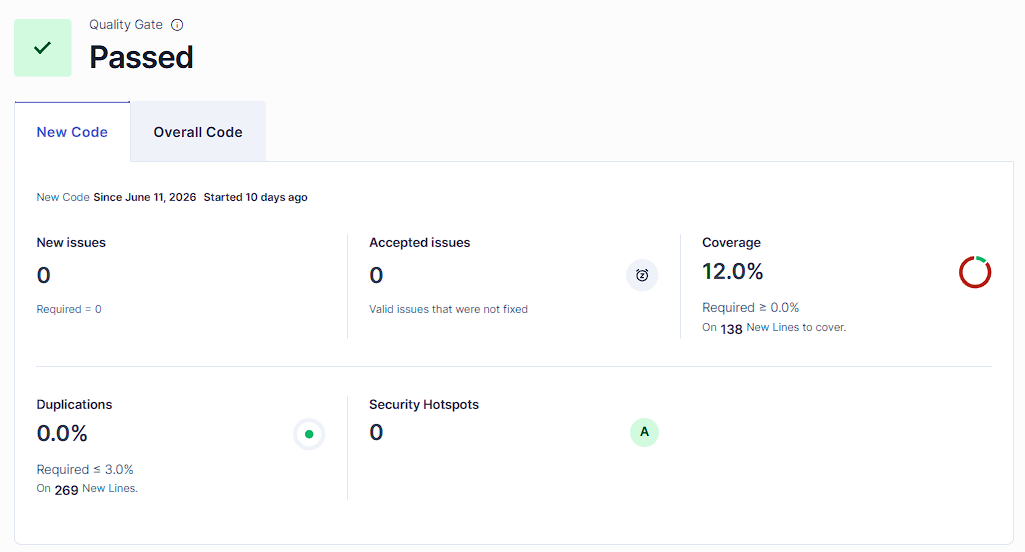
\includegraphics[width=0.8\textwidth]{images/sonarqube.png}
    \caption{Rapport SonarQube pour le projet GoatUdder}
    \label{fig:sonarqube}
\end{figure}

\section{ESLint}

Le linting est exécuté à chaque build CI pour chaque service:
\begin{itemize}[leftmargin=*]
    \item \texttt{goat-service/eslint.config.mjs}
    \item \texttt{rental-service/eslint.config.mjs}
\end{itemize}

\section{Code coverage de JEST et tests unitaires}

Pour `goat-service`:

\begin{figure}[H]
    \centering
    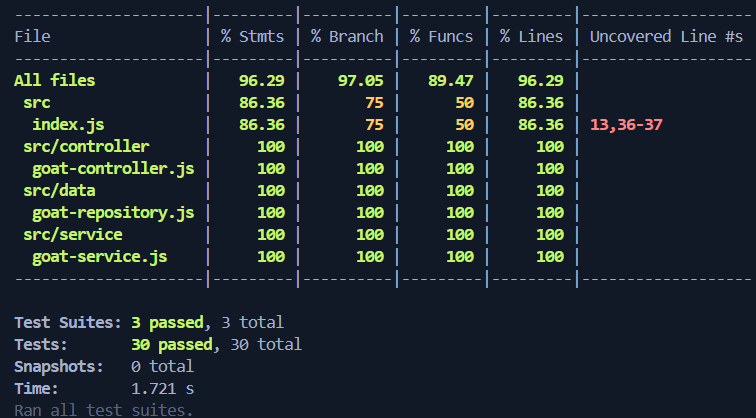
\includegraphics[width=0.8\textwidth]{images/goat-service-tests.png}
    \caption{Rapport de couverture de code pour le Goat Service}
    \label{fig:goat-service-coverage}
\end{figure}

Pour `rental-service`:

\begin{figure}[H]
    \centering
    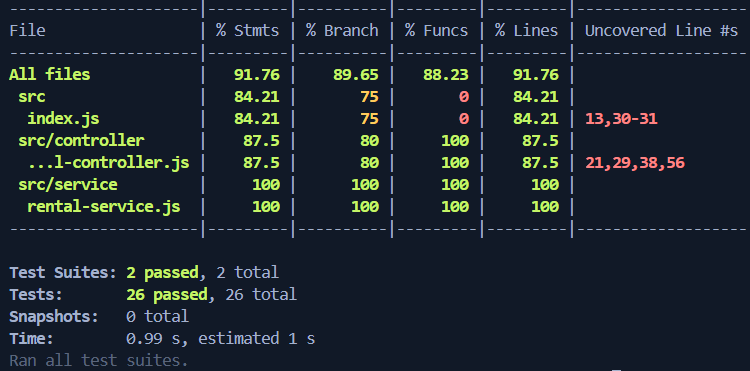
\includegraphics[width=0.8\textwidth]{images/rental-service-tests.png}
    \caption{Rapport de couverture de code pour le Rental Service}
    \label{fig:rental-service-coverage}
\end{figure}

\chapter{Captures d'écran des Google Labs}

Dashboard Google skills de MENON Valentin
\begin{figure}[H]
    \centering
    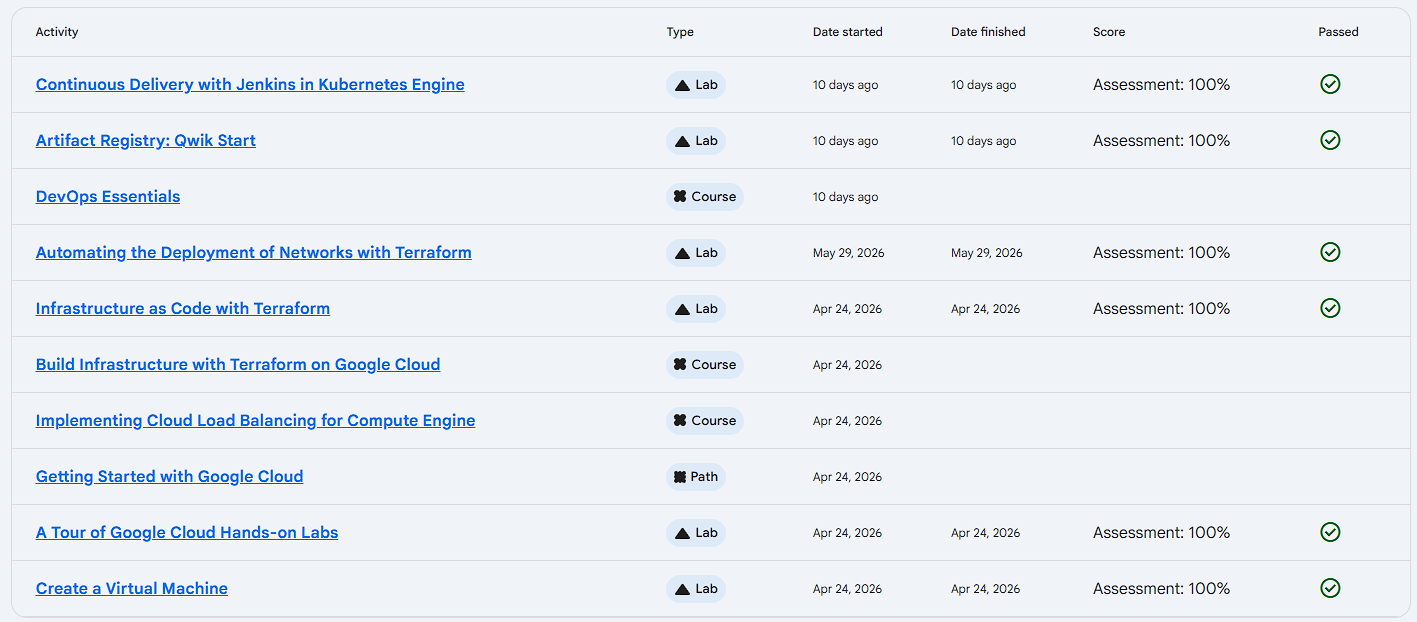
\includegraphics[width=0.8\textwidth]{images/google-skills-MENON.png}
    \caption{Dashboard Google Skills de MENON Valentin}
    \label{fig:google-skills-MENON}
\end{figure}

Dashboard Google skills de MASSINOND Matéo
\begin{figure}[H]
    \centering
    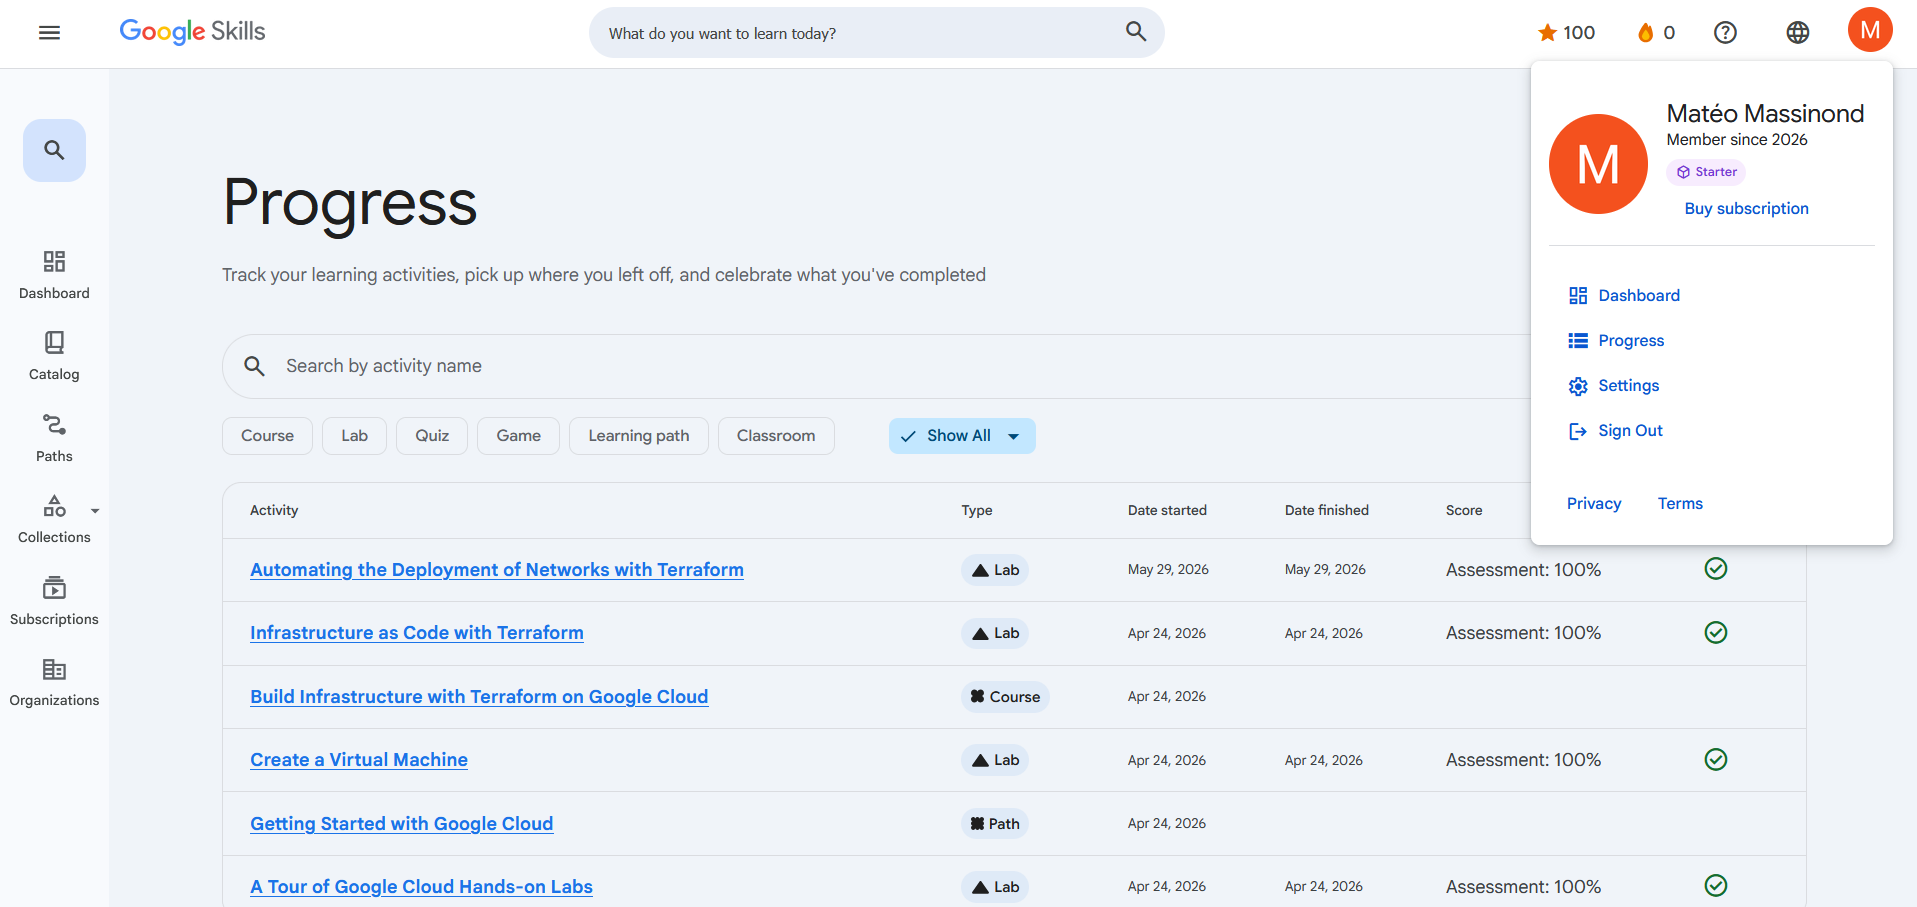
\includegraphics[width=0.8\textwidth]{images/google-skills-MASSINOND.png}
    \caption{Dashboard Google Skills de MASSINOND Matéo}
    \label{fig:google-skills-MASSINOND}
\end{figure}

\chapter{Accès aux Ressources}

\section{Dépôt Git (GitHub)}

Le repository est public et accessible à:

\begin{center}
    \url{https://github.com/GoatsSoftware/GoatUdder}
\end{center}

\section{Harbor Registry (Images Docker)}

\begin{center}
    \url{https://harbor.techops.tf/}
\end{center}

\textbf{Credentials:}
\begin{itemize}[leftmargin=*]
    \item \textbf{Username:} \texttt{bcharroux}
    \item \textbf{Password:}\\ \texttt{sLdRMfY722FBbvgOe8t6trSy2Efu4NaK8Tr7xRKQyaM8uCQvT3tg98gHyD7cr8iF}
\end{itemize}

\chapter{Conclusion}

Le projet \textbf{GoatUdder} respecte l'ensemble des exigences DevOps:
\begin{itemize}[leftmargin=*]
    \item $\checkmark$ Dépôt Git structuré
    \item $\checkmark$ Pipeline CI avec GitHub Actions
    \item $\checkmark$ Architecture en couches (Data, Service, Controller)
    \item $\checkmark$ 2 services back conteneurisés (Goat Service, Rental Service)
    \item $\checkmark$ Tests de toutes les couches (unitaires, mocks web)
    \item $\checkmark$ Couverture de code $\geq 80\%$
    \item $\checkmark$ Qualité logicielle (SonarQube, ESLint)
    \item $\checkmark$ Frontend web
    \item $\checkmark$ Base de données PostgreSQL
\end{itemize}

\end{document}